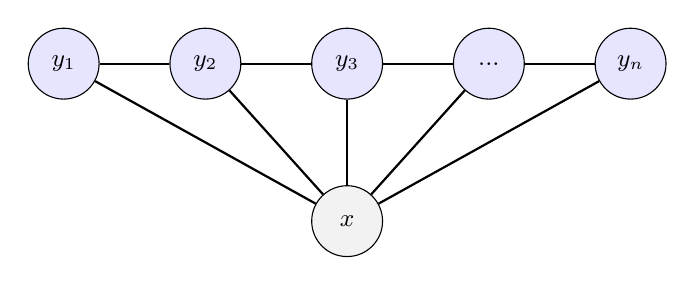
\begin{tikzpicture}[
    node distance=1.8cm,
    every node/.style={font=\small},
    obs/.style={circle, draw, minimum size=0.9cm, fill=gray!10},
    label/.style={circle, draw, minimum size=0.9cm, fill=blue!10},
    arrow/.style={->, thick, >=Stealth}
]

    % Labels above (y1 to y5)
    \node[label] (y1) at (0,0) {$y_1$};
    \node[label] (y2) [right of=y1] {$y_2$};
    \node[label] (y3) [right of=y2] {$y_3$};
    \node[label] (y4) [right of=y3] {...};
    \node[label] (y5) [right of=y4] {$y_n$};

    % Observed tokens (x1 to x5)
    \node[obs] (x) at (y3) [yshift=-2cm] {$x$};

    % Emission arrows (from x to y)
    \foreach \i in {1,...,5} {
        \draw[-, thick] (x) -- (y\i);
    }

    % Transition arrows (between y's)
    \foreach \i/\j in {1/2, 2/3, 3/4, 4/5} {
        \draw[-, thick] (y\i) -- (y\j);
    }

    % Caption
    % \node[align=center, below=1.2cm of x, font=\small] {
    %     Linear-chain CRF structure: emission edges (bottom-up) and transition edges (left-right).
    % };

\end{tikzpicture}

